A microring resonator is a waveguide closing on itself in a loop. This structure alone is isolated and it requires an additional straight waveguide at a distance \(g\) from the ring to couple light into it, as represented in Fig. \ref{fig:ring_design}. This is called all-pass configuration.

\begin{figure}[H]
    \centering
    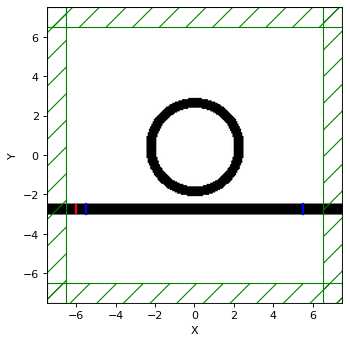
\includegraphics[width=0.6\linewidth]{Figures/ring_design.png}
    \caption{Design of the simulation of a microring resonator. The structure is composed of a ring and a waveguide both with refractive index \(n=1.7\). The waveguide and the ring have width \(w=0.5\ \mu m\) while the ring has an internal radius of \(r=2\ \mu m\). The gap between the guide and the ring is \(g=0.4\ \mu m\). All the simulations are done with a resolution \(r=16\) and PML of thickness \(1\ \mu m\)}
    \label{fig:ring_design}
\end{figure}

A Gaussian source (red line) is put inside the waveguide and then the field oscillating in the waveguide couples to the ring. Inside the ring, the field can be under the condition of constructive interference which corresponds to the resonance of the structure.

The source is set to a wavelength equal to a multiple of the perimeter of the ring and its width is about the FSR of the ring. The resulting transmission and reflection spectrum is shown in Fig. \ref{fig:ring_spectrum}. To find the resonance there are two possible methods: either find the minimum of the spectrum or use the Harminv algorithm (already implemented in MEEP) to find the resonance. The second method returns a resonance at \(\nu = 0.70 c/\mu m\).

\begin{figure}[H]
    \centering
    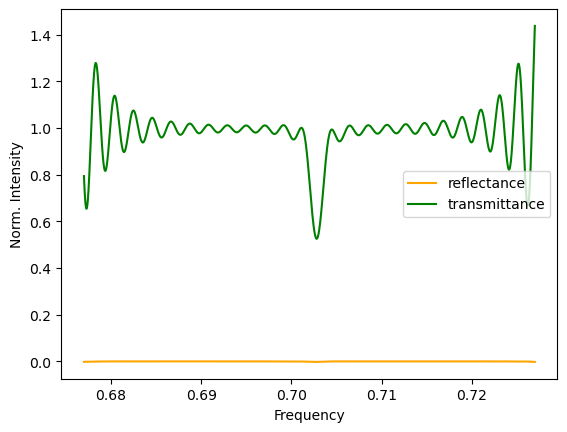
\includegraphics[width=0.8\linewidth]{Figures/ring_spectrum.png}
    \caption{Transmission and reflection spectra of the micro ring resonator coupled to a straight waveguide. The reflectivity is negligible, while transmittivity shows a resonance.}
    \label{fig:ring_spectrum}
\end{figure}

Switching to a continuous source and extracting the field's oscillations in the waveguide, it's possible to compute the phase difference between the field before and after the coupling with the ring. This is done by fitting the field in the two portions of the waveguide using sine functions as shown in Fig. \ref{fig:ring_phase_delay} and then subtracting the phases resulting from the fits.

\begin{figure}[H]
    \centering
    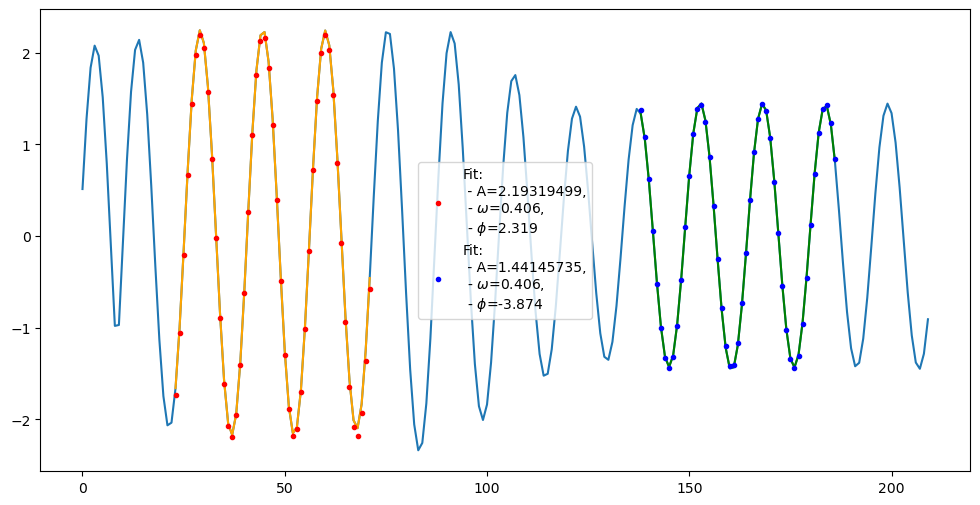
\includegraphics[width=0.8\linewidth]{Figures/ring_phase_delay.png}
    \caption{Electric field oscillating along the z-axis inside the waveguide. To obtain the phase difference produced by the coupling with the ring, two portions of the field are selected (orange and green portions) to be fitted and extract the phase difference between the field before and after the ring. The parameters resulting from the fit are reported in the legend, where the red dots represent the fit before the ring and the blue dots the fit after.}
    \label{fig:ring_phase_delay}
\end{figure}

In order to have a more precise transmission spectrum, the simulations are repeated with continuous sources at different frequencies. The spectrum is then fitted with a Lorentzian function to obtain the Q-factor of the ring resonator which is \(Q=365.5\). The resonance found here corresponds to the one computed from the Harminv algorithm.

\begin{figure}[H]
    \centering
    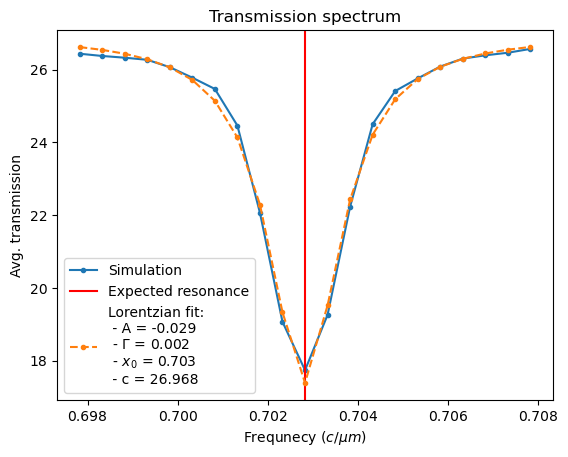
\includegraphics[width=0.7\linewidth]{Figures/ring_frequency_sweep.png}
    \caption{Transmission spectrum of the structure centered around the resonance and obtained by a sweep in the frequency of a continuous source.}
    \label{fig:ring_frequency_sweep}
\end{figure}

Another important behavior of the ring resonator is the change of phase difference in the three coupling regimes, namely the fields are in phase (\(\Delta \phi = 0\)) in under coupling, and they are in opposition to phase (\(\Delta \phi = \pi\)) in over coupling while they have a \(\Delta \phi = \frac{\pi}{2}\) phase difference in critical coupling.

The different coupling regimes depend on the gap between the ring and the straight waveguide. Repeating the simulations for values of the gap ranging from \(0.08\ \mu m\) to \(0.35\ \mu m\), the changes in phase difference are reported in Fig.\ref{fig:ring_phase_vs_gap}. 

The graph shows the over-coupling behavior for low values of the gap and the under-coupling behavior for the high values of the gap.

\begin{figure}[H]
    \centering
    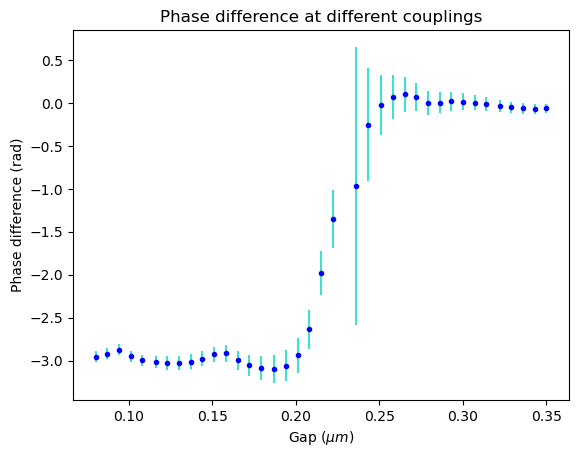
\includegraphics[width=0.7\linewidth]{Figures/ring_phase_vs_gap.png}
    \caption{Varion of the phase difference for a variation of the gap between the ring and the guide. The phase difference is obtained from the electric field fits, as reported above.}
    \label{fig:ring_phase_vs_gap}
\end{figure}